
\section{Equations of Motion \& Free Body Diagrams}

Equations of Motions and free body diagrams are the cornerstones of any dynamics. 
Determining how the vectors and forces is applied to the different bodies, a calculation of moment and force of each body can be managed.\\
Illustrated in figure \ref{fig:FBD} torques, lengths, different forces and vectors can be seen. By equating these, as seen in table \ref{tab:EoM}, every force and motion of each body is calculated.\\
These equations can then be used with the kinematics of the CrustCrawler, to determine position vectors, Torques and velocity vectors.

\begin{figure}[H]
    \centering
    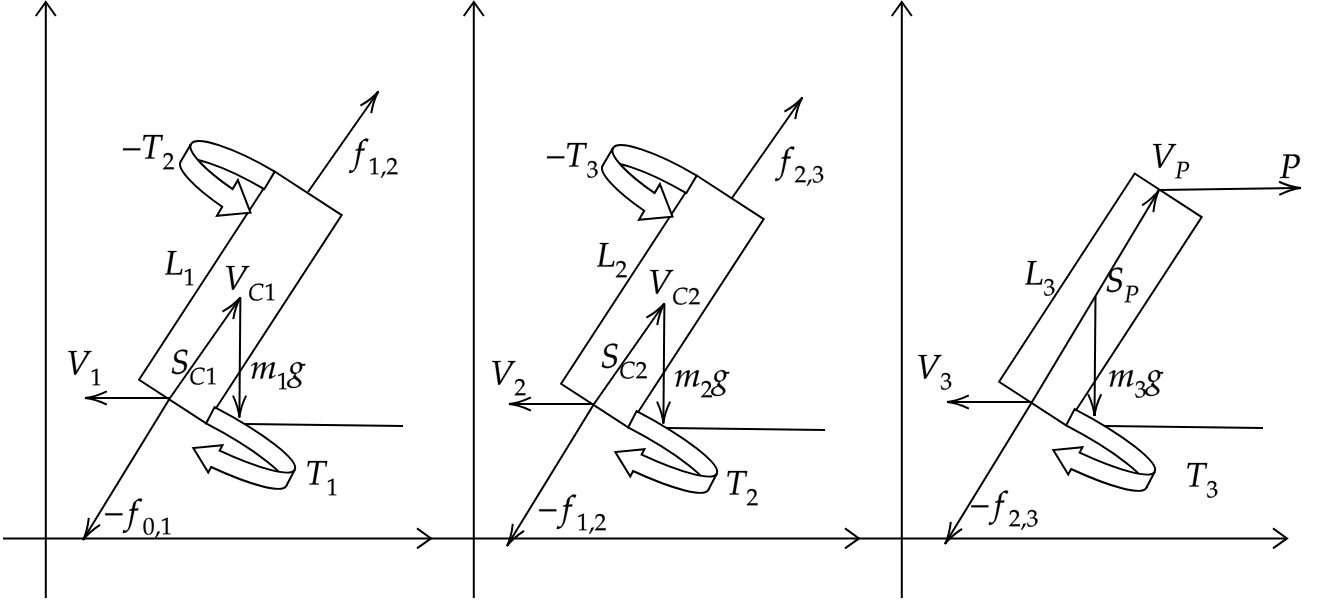
\includegraphics[width=14cm,height=5cm]{Figures/Technical_figures/FBD.png}
    \caption{Free body diagrams(FBD). Here all torques, lengths, different forces and vectors can be seen, by Equation these every force and motion of each body can be calculated}
    \label{fig:FBD}
\end{figure}

\begin{table}[H]
  \centering
\begin{tabular}{ |P{1.5cm}||P{4cm}||P{5cm}|}
 \hline
 \multicolumn{3}{|c|}{Equations of Motion} \\
 \hline
 Body & \(\sum F=ma\) & \(\sum M=I\alpha\)  \\
 \hline
 1 & \(-f_0_,_1+f_1_,_2+m_1g\) & \(\tau_1-\tau_2+(-S_C_1)\underline{X}(-f_0_,_1)+(S_1-S_C_1\underline{X}(f_1_,_2)\)  \\[7pt]
 \hline
 2 & \(-f_1_,_2+f_2_,_3+m_2g\) & \(\tau_2-\tau_3+(-S_C_2)\underline{X}(-f_1_,_2)+(S_2-S_C_2)\underline{X}(f_2_,_3)\) \\[7pt]
 \hline
 3 & \(-f_2_,_3+P\) & \(\tau_3+(-S_P)\underline{X}(-f_2_,_3)\) \\[7pt]
\hline
 \end{tabular}
 \caption{Equations of Motions}
    \label{tab:EoM}
\end{table}

\section{Recursive Newton-Euler}
The first approach which to determine dynamics of the CrustCrawler bodies is the recursive Newton-Euler through an inwards and outwards calculation. \\
Outward dynamics is the calculation of acceleration of each body from base to End-effector.\\
Inward dynamics is the calculation of forces on each body from End-effector to base.\\

\iffalse
\begin{table}[H]
  \centering
\begin{tabular}{|P{2cm}||P{4cm}||P{4cm}|}
 \hline
 \multicolumn{3}{|c|}{Preconditions of Recursive method} \\[7pt]
 \hline
& Angle     &   Angular velocity\\
Length & \(\theta\) & \(\omega\) \\
 \hline
  \hline
  & & \\
 L1 = 70 & \(\theta_1=\dfrac{\pi}{6}\) & \(\omega_1=\dfrac{\pi}{4}\) \\[1pt]
 & & \\
 \hline 
 & & \\
 L2 = 210 &\(\theta_2=\dfrac{\pi}{6}\) &\(\omega_2=\dfrac{5\pi}{12}\) \\[1pt]
 & & \\
 \hline
 & & \\
 L3 = 219 &\(\theta_3=\dfrac{-\pi}{3}\) &\(\omega_3=\dfrac{\pi}{12}\) \\[1pt]
& & \\
\hline
 \end{tabular}
 \label{EoM}
\end{table}
\fi

\begin{table}[H]
  \centering
\begin{tabular}{|P{4cm}||P{4cm}||P{4cm}|}
 \hline
 \multicolumn{3}{|c|}{Preconditions of Recursive method} \\[7pt]
 \hline
 Angle     &   Angular velocity  &  Reference velocity\\
 \(\theta\) & \(\omega\) & \(\dot\theta\)\\
 \hline
  \hline
  && \\
  \(\theta_1=\dfrac{\pi}{6}\) & \(\omega_1=\dfrac{\pi}{4}\) & \(\dot\theta_3=\dfrac{\pi}{4} \) \\[1pt]
  &&\\
 \hline 
  && \\
\(\theta_2=\dfrac{\pi}{6}\) &\(\omega_2=\dfrac{5\pi}{12}\) & \(\dot\theta_3=\dfrac{\pi}{6}\) \\[1pt]
  && \\
 \hline
  & &\\
 \(\theta_3=\dfrac{-\pi}{3}\) &\(\omega_3=\dfrac{\pi}{12}\) & \(\dot\theta_3=\dfrac{-\pi}{3}\) \\[1pt]
 & &\\
\hline
 \end{tabular}

 \caption{a stunning table} 
 \label{EoM}
\end{table}%\

\noindent
The first step is to find the position vectors of the bodies introduced in figure \ref{fig:FBD}.\\
This step is crucial for the recursive method, since the forces of the bodies will be added onto these vectors. To elaborate, it is known that forces on a long object will create more torque and more acceleration needed than a smaller object. Hereby the pre-conditions is of most importance to get the correct acceleration. \\
To find the vectors a simple mathematical approach is used:\\
finding the Center of Mass(C.O.M) vectors can be done by taking the length of the body and adding the different thetas in the x and y-axis direction. While the vector which runs through the whole body can be found using the same approach, but taking the whole length of the body.\\

 \begin{align}
     S_C_1&&=&&
\left[\begin{matrix}
    \dfrac{L_1}{2}\cdot \cos{\theta_1} \\[6pt]
    \dfrac{L_1}{2}\cdot \sin{\theta_1}
\end{matrix}\right]&&\Rightarrow&&
\left[\begin{matrix}
    30.312 \\[6pt]
    17.5
\end{matrix}\right]\\\notag 
\\
    S_1 &&=&&
\left[\begin{matrix}
    70\cdot \cos{\theta_1} \\[6pt]
    70\cdot \sin{\theta_1}
\end{matrix}\right]&&\Rightarrow&& 
\left[\begin{matrix}
    60.62 \\[6pt]
    35
\end{matrix}\right]\\\notag
\end{align}
\begin{align}
    \phi_1 &&=&& \theta_1+\theta_2 &&=&& \dfrac{\pi}{3}
\end{align}
\\

\begin{align} 
   S_C_2 &&=&&
\left[\begin{matrix}
    \dfrac{L_2}{2}\cdot \cos{\phi_1} \\[6pt]
    \dfrac{L_2}{2}\cdot \sin{\phi_1}
\end{matrix}\right]&&\Rightarrow&&
\left[\begin{matrix}
    52.50 \\[6pt]
    90.93
\end{matrix}\right]\\\notag
\\
    S_2 &&=&&
\left[\begin{matrix}
    210\cdot \cos{\phi_1\degree} \\[6pt]
    210\cdot \sin{\phi_1\degree}
\end{matrix}\right]&&\Rightarrow&&
\left[\begin{matrix}
    105 \\[6pt]
    181.87
\end{matrix}\right]\\\notag
\end{align}
\begin{align}
    \phi_2&&=&&\phi_1+\theta_3&&=&&0
\end{align}
\\
\begin{align}
    S_C_P &&=&&
\left[\begin{matrix}
    \dfrac{L_3}{2}\cdot \cos{\phi_2} \\[6pt]
    \dfrac{L_3}{2}\cdot \sin{\phi_2}
\end{matrix}\right]&&\Rightarrow&&
\left[\begin{matrix}
    109.5 \\[6pt]
    0
\end{matrix}\right]\\\notag
\\
    S_P &&=&&
\left[\begin{matrix}
    219\cdot \cos{\phi_2} \\
    219\cdot \sin{\phi_2}
\end{matrix}\right]&&\Rightarrow&&
\left[\begin{matrix}
    219 \\
    0
\end{matrix}\right]
\end{align}


The different velocities for each body can now be found, by using the outward recursive formulas:\\
As seen below there is three different points which the angular velocity takes place around. The first is the angular velocity, which is given by:\\
\begin{equation}\label{eq:W}
\omega_i=\omega_i-_1+\dot\theta_i
\end{equation}
The second, \(V_1\), calculating the velocity around the hinges and are given by:\\
\begin{equation}\label{eq:Vi}
V_i=V_i_-_1+\omega_i_-_1\cdot Z\underline{X}S_i
\end{equation}
The  second, \(V_C_1\), is the point which is the C.O.M of the body. By calculating around the point the angular velocity of the C.O.M can be found. The mathematically approach to this is given by:\\
\begin{equation}\label{eq:Vci}
V_C_i=V_i-_1+\omega_i-_1\cdot Z\underline{X}S_C_i
\end{equation}

\begin{align}
    V_1&&=&& &&=&&
\left[\begin{matrix}
    0\\
    0\\
    0
\end{matrix}\right]\\ V_C_1&&=&&V_1+\omega_1\cdot Z\underline{X}S_C_1&&=&&\left[\begin{matrix}
    -4.37\pi\\
    7.57\pi\\
    0
\end{matrix}\right]\\
    V_2&&=&&0+\omega_1\cdot Z\underline{X}S_1&&=&&
\left[\begin{matrix}
    -14.58\pi\\
    25.25\pi\\
    0
\end{matrix}\right]\\ V_C_2&&=&&V_2+\omega_2\cdot Z\underline{X}S_C_2&&=&&
\left[\begin{matrix}
   -45.80-37.88\pi \\
    79.32+21.87\pi\\
    0
\end{matrix}\right]\\
    V_3&&=&&V_2+\omega_2\cdot Z\underline{X}S_2&&=&&
\left[\begin{matrix}
    -45.80-15.15\pi\\
    79.32+8.70\pi\\
    0
\end{matrix}\right]\\ V_P&&=&&V_3&&=&&\left[\begin{matrix}
    45.80-15.15\pi\\
    79.32+8.70\pi\\
    0
\end{matrix}\right]
\end{align}
\\
Now that the velocities are known the accelerations of the different points can be found.\\
By proceeding to the acceleration, some alteration has to be taken into consideration. For example, the product of velocity on each point of interest, e-g \ref{eq:W}, \ref{eq:Vi} and \ref{eq:Vci}, will now be used as a reference point to get :

\begin{equation}
\dot\omega_i=\dot\omega_i-_1+\ddot\theta_i
\end{equation}

\begin{equation}
\dot{V}_i=\dot{V}_i_-_1+\dot\omega_i_-_1\cdot Z\underline{X}S_i_-_1+\omega_i_-_1\cdot Z\underline{X}(\omega_i_-_1\cdot\underline{X}S_i_-_1)
\end{equation}

\begin{equation}
\dot{V}_C_i=\dot{V}_i+\dot\omega_i\cdot Z\underline{X}S_C_i+\omega_i\cdot Z\underline{X}(\omega_i\cdot\underline{X}S_C_i)
\end{equation}
\\
In the next equations the result will be represented, not the calculation, since the course of action can be seen above.\\

\begin{align}
\dot\omega_1=\dfrac{\pi}{6}&&
    \dot{V}_1&&=
\left[\begin{matrix}
    0\\
    0\\
    0
\end{matrix}\right]&&,&&\dot{V}_C_1&&=\left[\begin{matrix}
    -27.40\\
    5.22\\
    0.
\end{matrix}\right]\\
\dot\omega_2=\dfrac{\pi}{12}&&
    \dot{V}_2&&=
\left[\begin{matrix}
    -55.33\\
    9.86\\
    0.
\end{matrix}\right]&&,&& \dot{V}_C_2&&=
\left[\begin{matrix}
   -167.99 \\
   -130.77\\
    0
\end{matrix}\right]\\
\dot\omega_3=\dfrac{\pi}{3}&&
    \Dot{V}_3&&=
\left[\begin{matrix}
    -282.37\\
    -271.72\\
    0
\end{matrix}\right]&&,&& \dot{V}_P&&=\left[\begin{matrix}
    -282.37\\
    -271.72\\
    0
\end{matrix}\right]
\end{align}
\\
\noindent
Finally the accelerations of the system can be used with the inward calculations and equations.\\
Equation \(f_i_-_1_,_i\), of the inwards, measures the applied forces of both inertial ,\(f_c_i\), and reaction forces \(f_i_,_i_+_1\).the equation is hereby given by:\\
\begin{equation}\label{eq:fi}
    f_i_-_1_,_i=f_c_i+f_i_,_i_+_1
\end{equation} 
Equation \ref{eq:Mi}, calculates the whole system of each body with angular accelerations and applied forces. This is equation is given by:\\
\begin{equation}\label{eq:Mi}
    M_i=M_c_i+m_i_+_1+S_c_i\underline{X}f_c_i+S_i\underline{X}f_i_,_i_+_i
\end{equation} 

Utilizing equation \ref{eq:fi} and \ref{eq:fi}, forces applied to the body at the hinge points can be found.\\

\begin{align}
    f_0_,_1=
\left[\begin{matrix}
    0\\
    0\\
    0
\end{matrix}\right]&& ,&&
M_1&&=&&\left[\begin{matrix}
    -4.37\pi\\
    7.57\pi\\
    0
\end{matrix}\right]\\
    f_1_,_2=
\left[\begin{matrix}
    -14.58\pi\\
    25.25\pi\\
    0
\end{matrix}\right]&&,&& 
M_2&&=&&
\left[\begin{matrix}
   -45.80-37.88\pi \\
    79.32+21.87\pi\\
    0
\end{matrix}\right]\\
    f_2_,_3=
\left[\begin{matrix}
    -45.80-15.15\pi\\
    79.32+8.70\pi\\
    0
\end{matrix}\right]&&,&& 
M_3&&=&&\left[\begin{matrix}
    45.80-15.15\pi\\
    79.32+8.70\pi\\
    0
\end{matrix}\right]
\end{align}
\\

\section{Lagrange}
Lagrange is the equation to use for measuring the kinetic energy T, which is the work the body needs to accelerate. While V, the potential energy, can measure the gravity potential \(V=M_g\cdot h\) and the elastic potential \(V=\dfrac{1}{2}\cdot x^2\). Those two equation subtracted with each other gives the Lagrangian 

\begin{equation}
    \mathcal{L}=T-V
\end{equation}

\subsection*{Lagrange equation}

The Lagrange eq. states the following, The time derivative of the partial derivative Lagrangian with respect to the $\Dot{q}_i$ (generalised velocity) minus the partial derivative Lagrangian with respect to the $q_i$ (generalised force) equals:
\begin{equation}
    Q_i = \frac{d}{dt}(\frac{\partial\mathcal{L}}{\parital \Dot{q_i}})-\frac{\partial\mathcal{L}}{\parital q_i}
\end{equation}
$Q_i$ is the generalised force for one body. The \textit{i} is referring to the D.O.F of the system, meaning that in the case of the Crustcrawler, there is the need to compute this 3 times with respect to the 3 D.O.F. as stated below by the known thetas:\\

\begin{align*}
    Torque\ 1\ (\tau_1):&& \dfrac{d}{dt}\cdot\dfrac{\delta L_3}{\delta\dot{\theta_1}}-\dfrac{\delta L_3}{\delta\theta_1}&&=&&-4.8667Nm\\
    Torque\ 2\ (\tau_2):&& \dfrac{d}{dt}\cdot\dfrac{\delta L_3}{\delta \dot{\theta_2}}-\dfrac{\delta L_3}{\delta\theta_2}&&=&& 1.757Nm\\
    torque\ 3\ (\tau_3):&&\dfrac{d}{dt}\cdot\dfrac{\delta L_3}{\delta \dot{\theta_3}}-\dfrac{\delta L_3}{\delta\theta_3}&&=&&-1.663Nm
\end{align*}
\\

By known theory Lagranian law, \(q=\theta, and \theta=\tau\), therefore both torque and general force can be equated by this single equation.
 
 \section{Jacobians}
 In vector calculus the concept of Jacobians refers to a matrix of first order partial derivatives from sets of multivariable functions. Given a set of n functions y=f(x) with n variables x\_n.\\

\begin{equation}
    y_1=f_1(x_1 \dots x_n)\\
    y_2=f_2(x_1 \dots x_n);\\
    \\
    y_n=f_n(x_1 \dots x_n);

\end{equation}

then the Jacobian matrix is:\\ 
\begin{equation}
\begin{bmatrix}
 \dfrac{\partial y_1}{\partial x_1} & \dots &  \dfrac{\partial y_1}{\partial x_n} \\
\dots & \dots & \dots \\
 \dfrac{\partial y_n}{\partial x_1} &  \dots &  \dfrac{\partial y_n}{\partial x_n} 
\end{bmatrix} 
\end{equation}

Jacobians are used to describe the change in a transformation matrix. This means it is used to describe the rotational change of a point in Cartesian space after a transformation matrix is implemented.


\subsection{Robot Jacobian}
In robot kinematics, \textit{"Jacobians"} is an important concept. 
It is used to show a relation between the manipulator end-effectors velocity and the joint velocities.\cite{ShaopingLN}
\begin{equation}\label{end.eff.vel}
    \dot x = J \cdot \dot{\theta}
\end{equation}
The equation \ref{end.eff.vel} shows the relation of the end-effector velocity, the joint velocity and the manipulator Jacobian. This means the \textit{"the velocity of the end effector of a robot is the linear mapping of the joint velocities" \cite{ShaopingLN}}\\

\subsection{Singularities}
If  the Jacobian determinant is zero, then the manipulator will reach a singularity. 
\begin{equation}
    det(J)=0
\end{equation}
This means the manipulator will experience system difficulties, this could be if the manipulators joints are perpendicular, then there are too many solutions for one point, to decide a given motion.